\documentclass{article} % For LaTeX2e
\usepackage{nips2013submit_e,times}
\usepackage{hyperref}
\usepackage{url}
\usepackage{graphicx}
\usepackage{amsmath}
\usepackage{caption}
\usepackage{subcaption}
\usepackage{color}
%\documentstyle[nips2013submit_09,times,art10]{article} % For LaTeX 2.09


\title{10-601b: Mid-term report}


\author{
David S.~Hippocampus\thanks{ Use footnote for providing further information
about author (webpage, alternative address)---\emph{not} for acknowledging
funding agencies.} \\
Department of Computer Science\\
Cranberry-Lemon University\\
Pittsburgh, PA 15213 \\
\texttt{hippo@cs.cranberry-lemon.edu} \\
\And
Coauthor \\
Affiliation \\
Address \\
\texttt{email} \\
\AND
Coauthor \\
Affiliation \\
Address \\
\texttt{email} \\
\And
Coauthor \\
Affiliation \\
Address \\
\texttt{email} \\
\And
Coauthor \\
Affiliation \\
Address \\
\texttt{email} \\
(if needed)\\
}

% The \author macro works with any number of authors. There are two commands
% used to separate the names and addresses of multiple authors: \And and \AND.
%
% Using \And between authors leaves it to \LaTeX{} to determine where to break
% the lines. Using \AND forces a linebreak at that point. So, if \LaTeX{}
% puts 3 of 4 authors names on the first line, and the last on the second
% line, try using \AND instead of \And before the third author name.

\newcommand{\fix}{\marginpar{FIX}}
\newcommand{\new}{\marginpar{NEW}}

%\nipsfinalcopy % Uncomment for camera-ready version

\begin{document}


\maketitle

\begin{abstract}
    In this report, we list the results we've achieved for classifying the subset of the CIFAR-10 dataset. We use the K-nearest neighbours and SVM to achieve an accuracy of X\% and Y\% respectively.\\
\end{abstract}

\section{Introduction}
    \begin{itemize}
        \item The problem statement
        \item The Cifar-10 dataset
        \item Our approaches
    \end{itemize}

\section{Exploratory data analysis}
    \begin{itemize}
        \item How we intend to test our results
        \item Distribution of the various labels
        \item Color variance of the dataset
        \item Average image of each label class
        \item Average HOG in each label class
    \end{itemize}

    \begin{figure}[h]
        \centering
        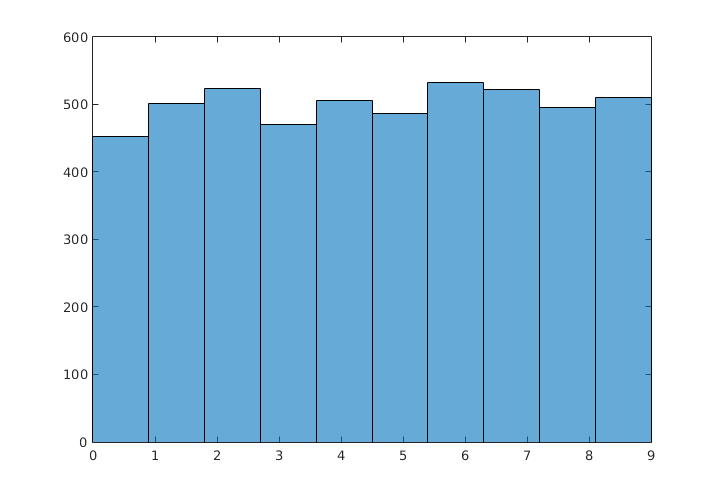
\includegraphics[width=.4\linewidth]{label-distribution.png}
        \caption{Distribution of the ground truth labels}
    \end{figure}
    \begin{figure}[h]
        \centering
        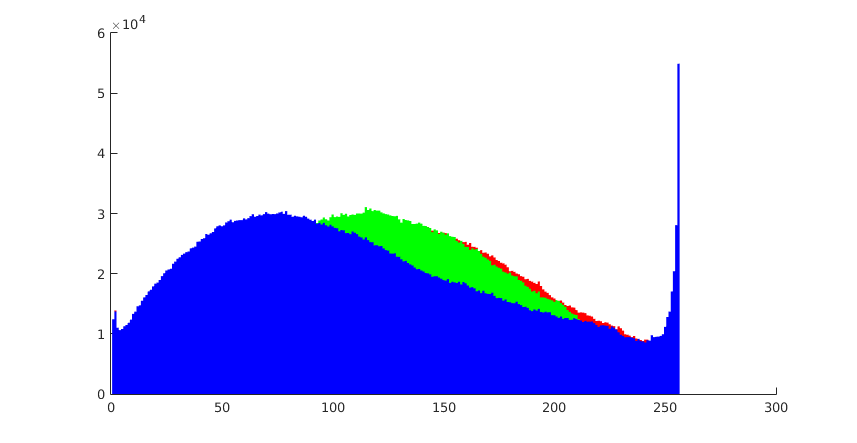
\includegraphics[width=.4\linewidth]{hist-overall.png}
        \caption{Distribution of RGB across all 5000 images}
    \end{figure}
    \begin{figure}[h]
        \begin{subfigure}{\linewidth}
            \centering
            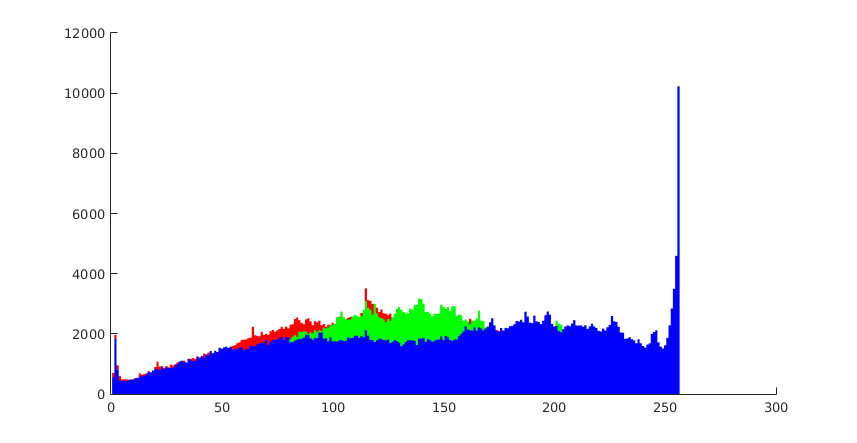
\includegraphics[width=.18\linewidth]{hist-class-0.png}
            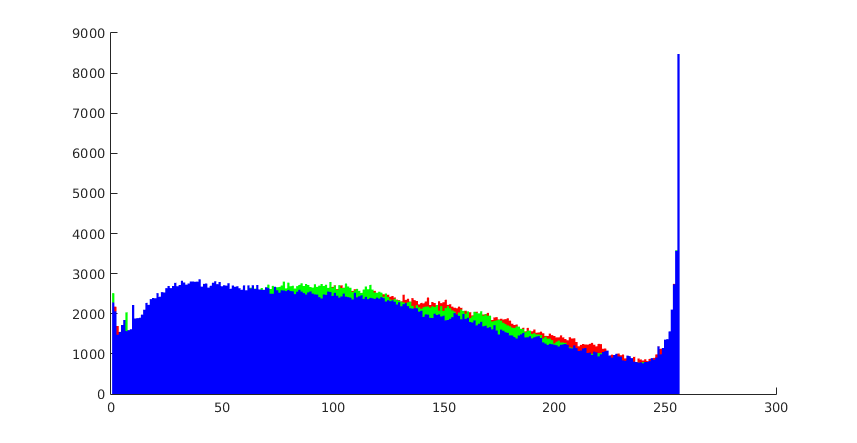
\includegraphics[width=.18\linewidth]{hist-class-1.png}
            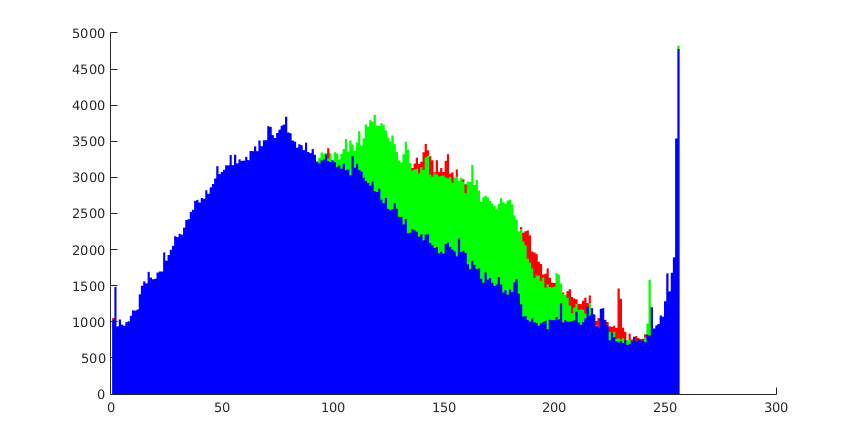
\includegraphics[width=.18\linewidth]{hist-class-2.png}
            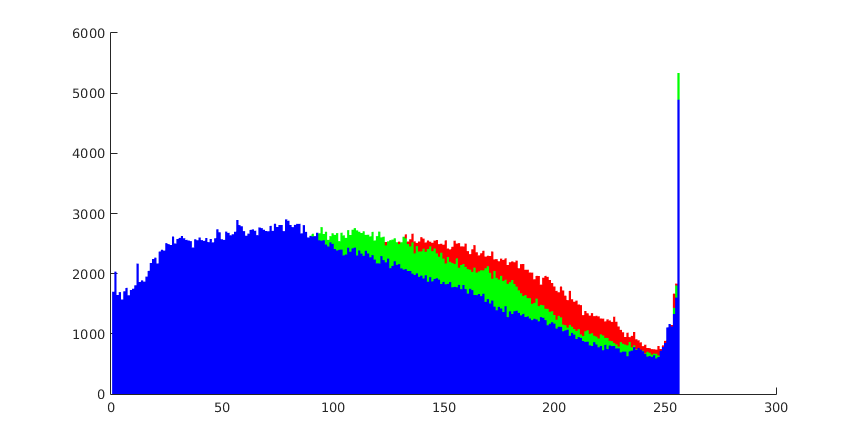
\includegraphics[width=.18\linewidth]{hist-class-3.png}
            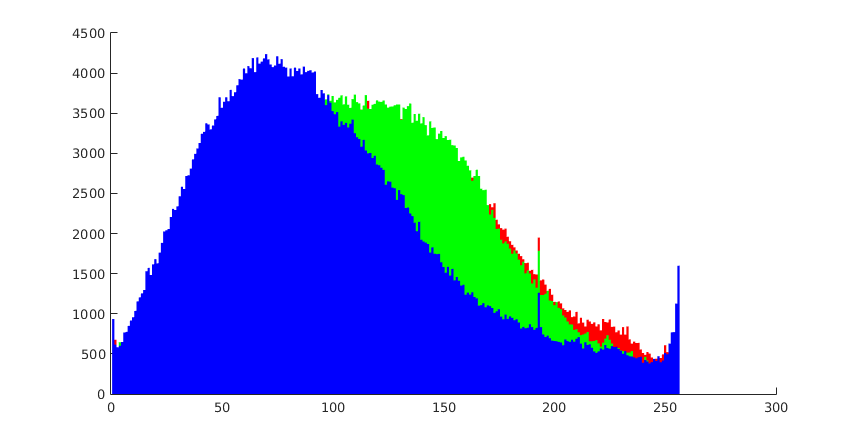
\includegraphics[width=.18\linewidth]{hist-class-4.png}
        \end{subfigure}
        \begin{subfigure}{\linewidth}
            \centering
            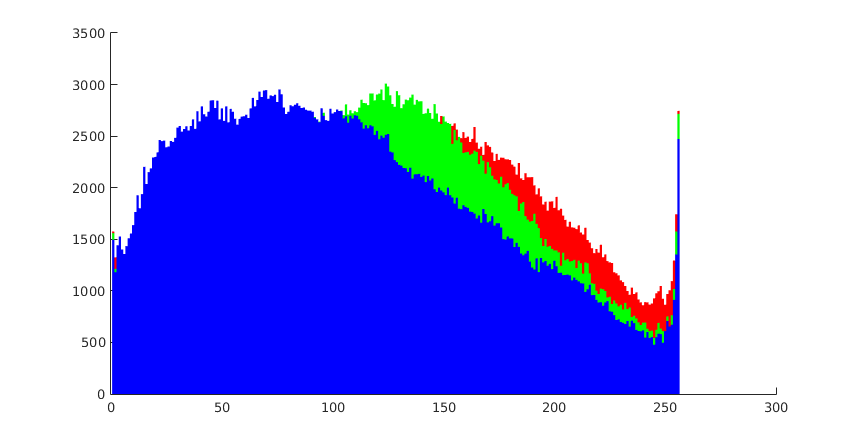
\includegraphics[width=.18\linewidth]{hist-class-5.png}
            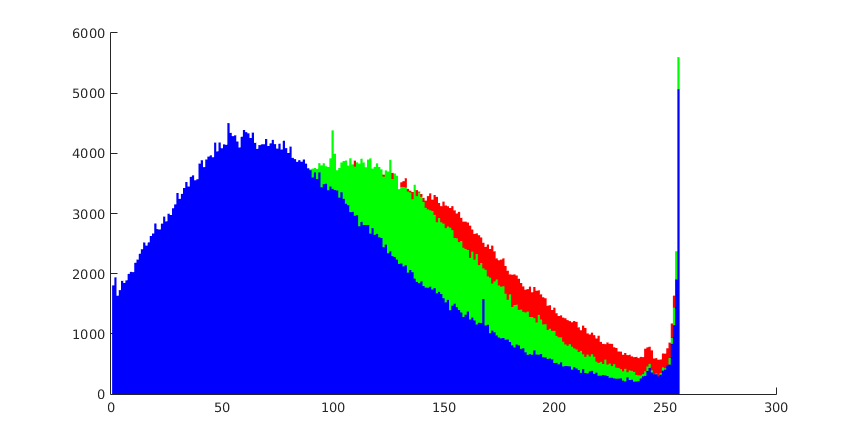
\includegraphics[width=.18\linewidth]{hist-class-6.png}
            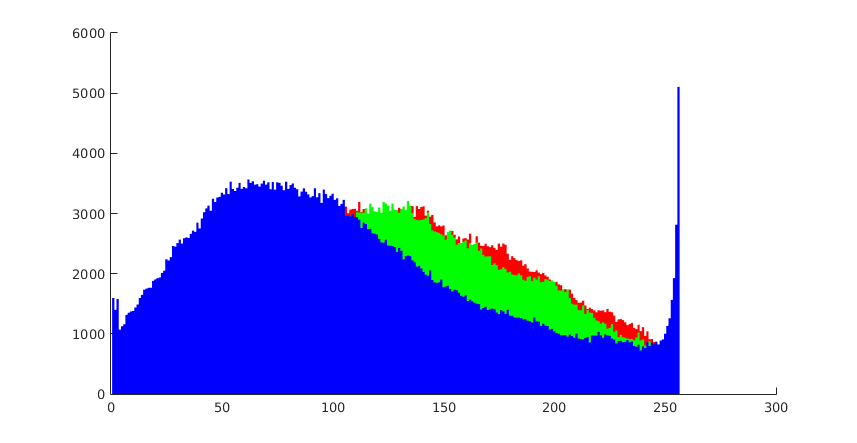
\includegraphics[width=.18\linewidth]{hist-class-7.png}
            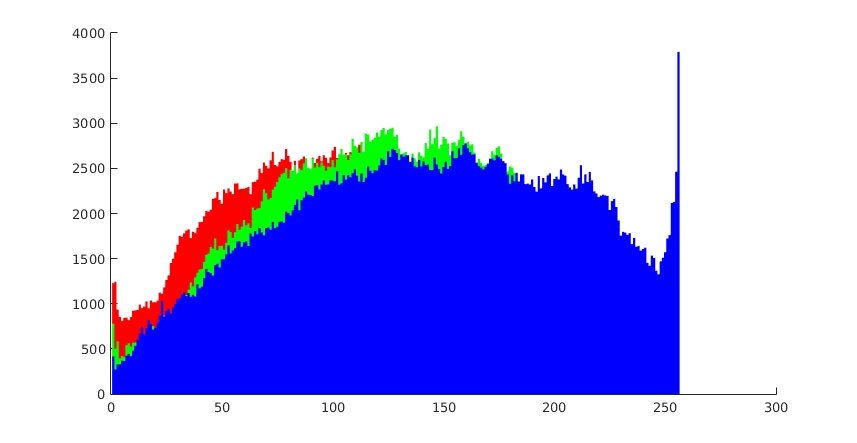
\includegraphics[width=.18\linewidth]{hist-class-8.png}
            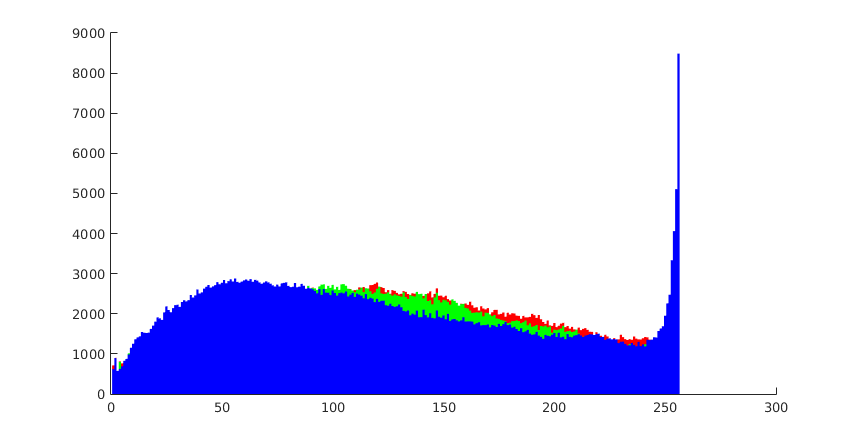
\includegraphics[width=.18\linewidth]{hist-class-9.png}
        \end{subfigure}
        \caption{RGB histogram for each class}
    \end{figure}
    

\section{Classification with K-means and K-Nearest Neighbours}
    \subsection{K-Means} % (fold)
    \label{ssub:K-Means}
        \begin{itemize}
            \item K-means on raw images
            \item K-means on filtered images (filter banks, gabor filters)
            \item K-means speed as the number of clusters increase
        \end{itemize}
    % subsubsection K-Means (end)

    %%%%%%%%%%%%%%%%%%%%%%%%%%%%%%%%%%%%%%%%%%
    \subsection{K-Nearest Neighbours} % (fold)
    \label{sub:K-Nearest Neighbours}
        \begin{itemize}
            \item Given the terrible training speed
            \item Using filtered images
            \item Classification speed
            \item Switching to HOG classifiers
        \end{itemize}
    % subsection K-Nearest Neighbours (end)

    %%%%%%%%%%%%%%%%%%%%%%%%%%%%%%%%%%%%%%%%%%
    \subsection{Results} % (fold)
    \label{sub:Results}
    
    % subsection Results (end)

\section{Support vector machines}
    \begin{itemize}
        \item The outline goes here?
        \item More outline here
    \end{itemize}

    %%%%%%%%%%%%%%%%%%%%%%%%%%%%%%%%%%%%%%%%%%
    \subsection{Results} % (fold)
    \label{sub:Results}
    
    % subsection Results (end)

% FIGURE SAMPLE
\begin{figure}[h]
    \begin{center}
    %\framebox[4.0in]{$\;$}
    \fbox{\rule[-.5cm]{0cm}{4cm} \rule[-.5cm]{4cm}{0cm}}
    \end{center}
    \caption{Sample figure caption.}
\end{figure}

% TABLE SAMPLE
\begin{table}[t]
    \caption{Sample table title}
    \begin{center}
        \begin{tabular}{ll}
        \multicolumn{1}{c}{\bf PART}  &\multicolumn{1}{c}{\bf DESCRIPTION}
        \\ \hline \\
        Dendrite         &Input terminal \\
        Axon             &Output terminal \\
        Soma             &Cell body (contains cell nucleus) \\
        \end{tabular}
    \end{center}
\end{table}

\subsubsection*{Acknowledgments}

Use unnumbered third level headings for the acknowledgments. All
acknowledgments go at the end of the paper. Do not include 
acknowledgments in the anonymized submission, only in the 
final paper. 

\subsubsection*{References}

References follow the acknowledgments. Use unnumbered third level heading for
the references. Any choice of citation style is acceptable as long as you are
consistent. It is permissible to reduce the font size to `small' (9-point) 
when listing the references. {\bf Remember that this year you can use
a ninth page as long as it contains \emph{only} cited references.}

\small{
[1] Alexander, J.A. \& Mozer, M.C. (1995) Template-based algorithms
for connectionist rule extraction. In G. Tesauro, D. S. Touretzky
and T.K. Leen (eds.), {\it Advances in Neural Information Processing
Systems 7}, pp. 609-616. Cambridge, MA: MIT Press.

[2] Bower, J.M. \& Beeman, D. (1995) {\it The Book of GENESIS: Exploring
Realistic Neural Models with the GEneral NEural SImulation System.}
New York: TELOS/Springer-Verlag.

[3] Hasselmo, M.E., Schnell, E. \& Barkai, E. (1995) Dynamics of learning
and recall at excitatory recurrent synapses and cholinergic modulation
in rat hippocampal region CA3. {\it Journal of Neuroscience}
{\bf 15}(7):5249-5262.
}

\end{document}
